\chapter{MCP and external tool integration}

\section{Engineering principles}

MCP connects a host application to external capabilities through clients and servers. Tools expose callable operations; resources expose data; prompts expose reusable interaction templates. Protocol version and transport support must be negotiated rather than assumed. Local stdio and network transports have different trust and authentication properties. A valid schema is not authorization, and a server tool description may contain hostile content.\src{M1,O8,A7}

\section{Implementation approach}

Start with a read-only service that returns an allowlisted policy summary. Validate parameters and limit result size. Deploy under a task-scoped identity; for remote HTTP, validate the applicable authorization requirements, audience and scopes. Map repository reads, issue reads, documentation search, CI status and scanner findings to separate least-privilege endpoints. Keep mutation operations behind explicit approval and server-side policy.

\section{Verification and limitations}

Use a negative test for unknown policy IDs and unauthorized objects. Confirm server provenance and pinned dependencies. The local example uses the Python MCP SDK interface and is syntax-checked only; protocol handshake and installed SDK version require live testing.

Figure~\ref{fig:d9} illustrates the conceptual flow from Agent host to Scoped service. The edges describe the proposed integration or control relationship, not undocumented internal calls.

\begin{figure}[htbp]\centering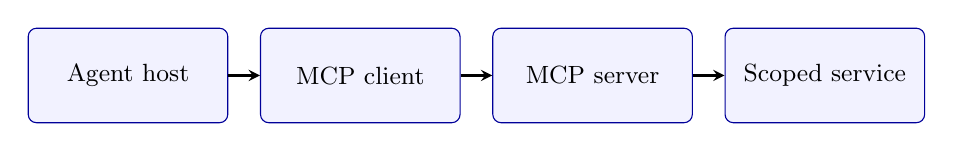
\begin{tikzpicture}[nodebox/.style={draw=blue!60!black,fill=blue!5,rounded corners=3pt,minimum height=12mm,text width=23mm,align=center,font=\small},>=stealth]
\node[nodebox] (n0) at (0.00,0.00) {Agent host};
\node[nodebox] (n1) at (2.95,0.00) {MCP client};
\node[nodebox] (n2) at (5.90,0.00) {MCP server};
\node[nodebox] (n3) at (8.85,0.00) {Scoped service};
\draw[->,thick] (n0.east) -- (n1.west);
\draw[->,thick] (n1.east) -- (n2.west);
\draw[->,thick] (n2.east) -- (n3.west);
\end{tikzpicture}
\caption{MCP integration (conceptual view).}\label{fig:d9}\end{figure}

\section{Chapter conclusion}

Apply the stated verification criteria before expanding the scope of this workflow. Record deviations, evidence and unresolved risks in the task record.
